%%%%%%%%%%%%%%%%%%%%%%%%%%%%%%%%%%%%%%%%%%%%%%%%%%%%%%%%%%%%%%%%%%%%%%%%%%%%%%%%%%%%%%%%%%%%%%%%%%%%%%%
%%													%%
%% 	DIPLOMOVÁ PRÁCE -  Rozšíření zásuvného modulu QGIS pro zpracování GTFS o vizualizaci tarifních pásem PID		%%
%% 				Adam Kulhavý							%%
%%													%%
%% pro formátování využita šablona: http://geo3.fsv.cvut.cz/kurzy/mod/resource/view.php?id=775 	%%
%%													%%
%%%%%%%%%%%%%%%%%%%%%%%%%%%%%%%%%%%%%%%%%%%%%%%%%%%%%%%%%%%%%%%%%%%%%%%%%%%%%%%%%%%%%%%%%%%%%%%%%%%%%%% 

\documentclass[%
  12pt,         			% Velikost základního písma je 12 bodů
  a4paper,      			% Formát papíru je A4
  oneside,       			% Oboustranný tisk
  pdftex,				    % překlad bude proveden programem 'pdftex' do PDF
%%%  draft
]{report}       			% Dokument třídy 'zpráva'
%

\newcommand{\Fbox}[1]{\fbox{\strut#1}}

\usepackage[czech, english]{babel}	% použití češtiny, angličtiny
\usepackage[utf8]{inputenc}		% Kódování zdrojových souborů je UTF8

\usepackage[square,sort,comma,numbers]{natbib}

\usepackage{caption}
\usepackage{subcaption}
\captionsetup{font=small}
\usepackage{enumitem} 
\setlist{leftmargin=*} % bez odsazení

\makeatletter
\setlength{\@fptop}{0pt}
\setlength{\@fpbot}{0pt plus 1fil}
\makeatletter

\usepackage[dvips]{graphicx}   
\usepackage{color}
\usepackage{transparent}
\usepackage{wrapfig}
\usepackage{float} 

\usepackage{cmap}           
\usepackage[T1]{fontenc}    

\usepackage{setspace}
\onehalfspacing 
\usepackage{etoolbox}
\AtBeginEnvironment{quote}{\singlespacing\small}

\usepackage{textcomp}
\usepackage[compact]{titlesec}
\usepackage{amsmath}
\addtolength{\jot}{1em} 

\usepackage{chngcntr}
\counterwithout{footnote}{chapter}

\usepackage{acronym}

\usepackage[
    unicode,                
    breaklinks=true,        
    hypertexnames=false,
    colorlinks=true, % true for print version
    citecolor=black,
    filecolor=black,
    linkcolor=black,
    urlcolor=black
]{hyperref}         

\usepackage{url}
\usepackage{fancyhdr}
%\usepackage{algorithmic}
\usepackage{algorithm}
\usepackage{algcompatible}
\renewcommand{\ALG@name}{Pseudokód}% Update algorithm name
\def\ALG@name{Pseudokód}

\usepackage{dirtree}
\usepackage{booktabs}
\usepackage{graphicx}
\usepackage[table,xcdraw]{xcolor}
\usepackage{array}

\usepackage[
  cvutstyle,          
  diploma           
]{thesiscvut}


\newif\ifweb
\ifx\ifHtml\undefined % Mimo HTML.
    \webfalse
\else % V HTML.
    \webtrue
\fi 

\renewcommand{\figurename}{Obrázek}
\def\figurename{Obrázek}

%%%%%%%%%%%%%%%%%%%%%%%%%%%%%%%%%%%%%%%%%%%%%%%%%%%%%%%%%%%%%%%%%
%%%%%%%%%%% Definice informací o dokumentu  %%%%%%%%%%%%%%%%%%%%%
%%%%%%%%%%%%%%%%%%%%%%%%%%%%%%%%%%%%%%%%%%%%%%%%%%%%%%%%%%%%%%%%%

%% Název práce
\nazev{Tvorba webové aplikace pro projekt Viskalia}
{Web application for Viskalia project}

%% Jméno a příjmení autora
\autor{Bc.~Adam}{Kulhavý}

%% Jméno a příjmení vedoucího práce včetně titulů
\garant{Ing.~Martin~Landa,~Ph.D.}

%% Označení programu studia
\programstudia{Geodézie a~kartografie}{}

%% Označení oboru studia
\oborstudia{Geomatika}{}

%% Označení ústavu
\ustav{Katedra geomatiky}{}

%% Rok obhajoby
\rok{2021}

%Mesic obhajoby
\mesic{červen}

%% Místo obhajoby

\misto{Praha}

%% Abstrakt
\abstrakt {Tato diplomová práce se zabývá vytvořením webové aplikace pro projekt Viskalia. 
Webová aplikace je tvořena v Python frameworku Django s připojením k databázovému systému MariaDB.
Aplikace je tvořena v administrátorském prostředí, kde je optimalizována dle potřeb projektu.
Jedním z cílů je také automatizované nasazení aplikace a databáze v izolovaném prostředí.}
	      {This Master's thesis deals with the creation of a web application for the Viskalia project. The web application is created in Python framework named Django with a connection to the MariaDB database. The application is developed in an administration environment adapted to the needs of the project. One of the goals is to create an automated deployment for application and database in an isolated environment}

%% Klíčová slova
\klicovaslova
{Python, Django, Webová aplikace, Docker, MariaDB, Viskalia}
{Python, Django, Web application, Docker, MariaDB, Viskalia}

%%%%%%%%%%%%%%%%%%%%%%%%%%%%%%%%%%%%%%%%%%%%%%%%%%%%%%%%%%%%%%%%%%%%%%%%

%%%%%%%%%%%%%%%%%%%%%%%%%%%%%%%%%%%%%%%%%%%%%%%%%%%%%%%%%%%%%%%%%%%%%%%%
%% Nastavení polí ve Vlastnostech dokumentu PDF
%%%%%%%%%%%%%%%%%%%%%%%%%%%%%%%%%%%%%%%%%%%%%%%%%%%%%%%%%%%%%%%%%%%%%%%%
\nastavenipdf
%%%%%%%%%%%%%%%%%%%%%%%%%%%%%%%%%%%%%%%%%%%%%%%%%%%%%%%%%%%%%%%%%%%%%%%
\DeclareUnicodeCharacter{2212}{-}
%%% Začátek dokumentu
\begin{document}

\catcode`\-=12  % pro vypnuti aktivniho znaku '-' pouzivaneho napr. v \cline 

% aktivace záhlaví
\zahlavi

% předefinování vzhledu záhlaví
\renewcommand{\chaptermark}[1]{%
	\markboth{\MakeUppercase
	{%
	\thechapter.%
	\ #1}}{}}

% Vysázení přebalu práce
%\vytvorobalku

% Vysázení titulní stránky práce
\vytvortitulku

% Vysázení listu zadani
\stranka{}%
	{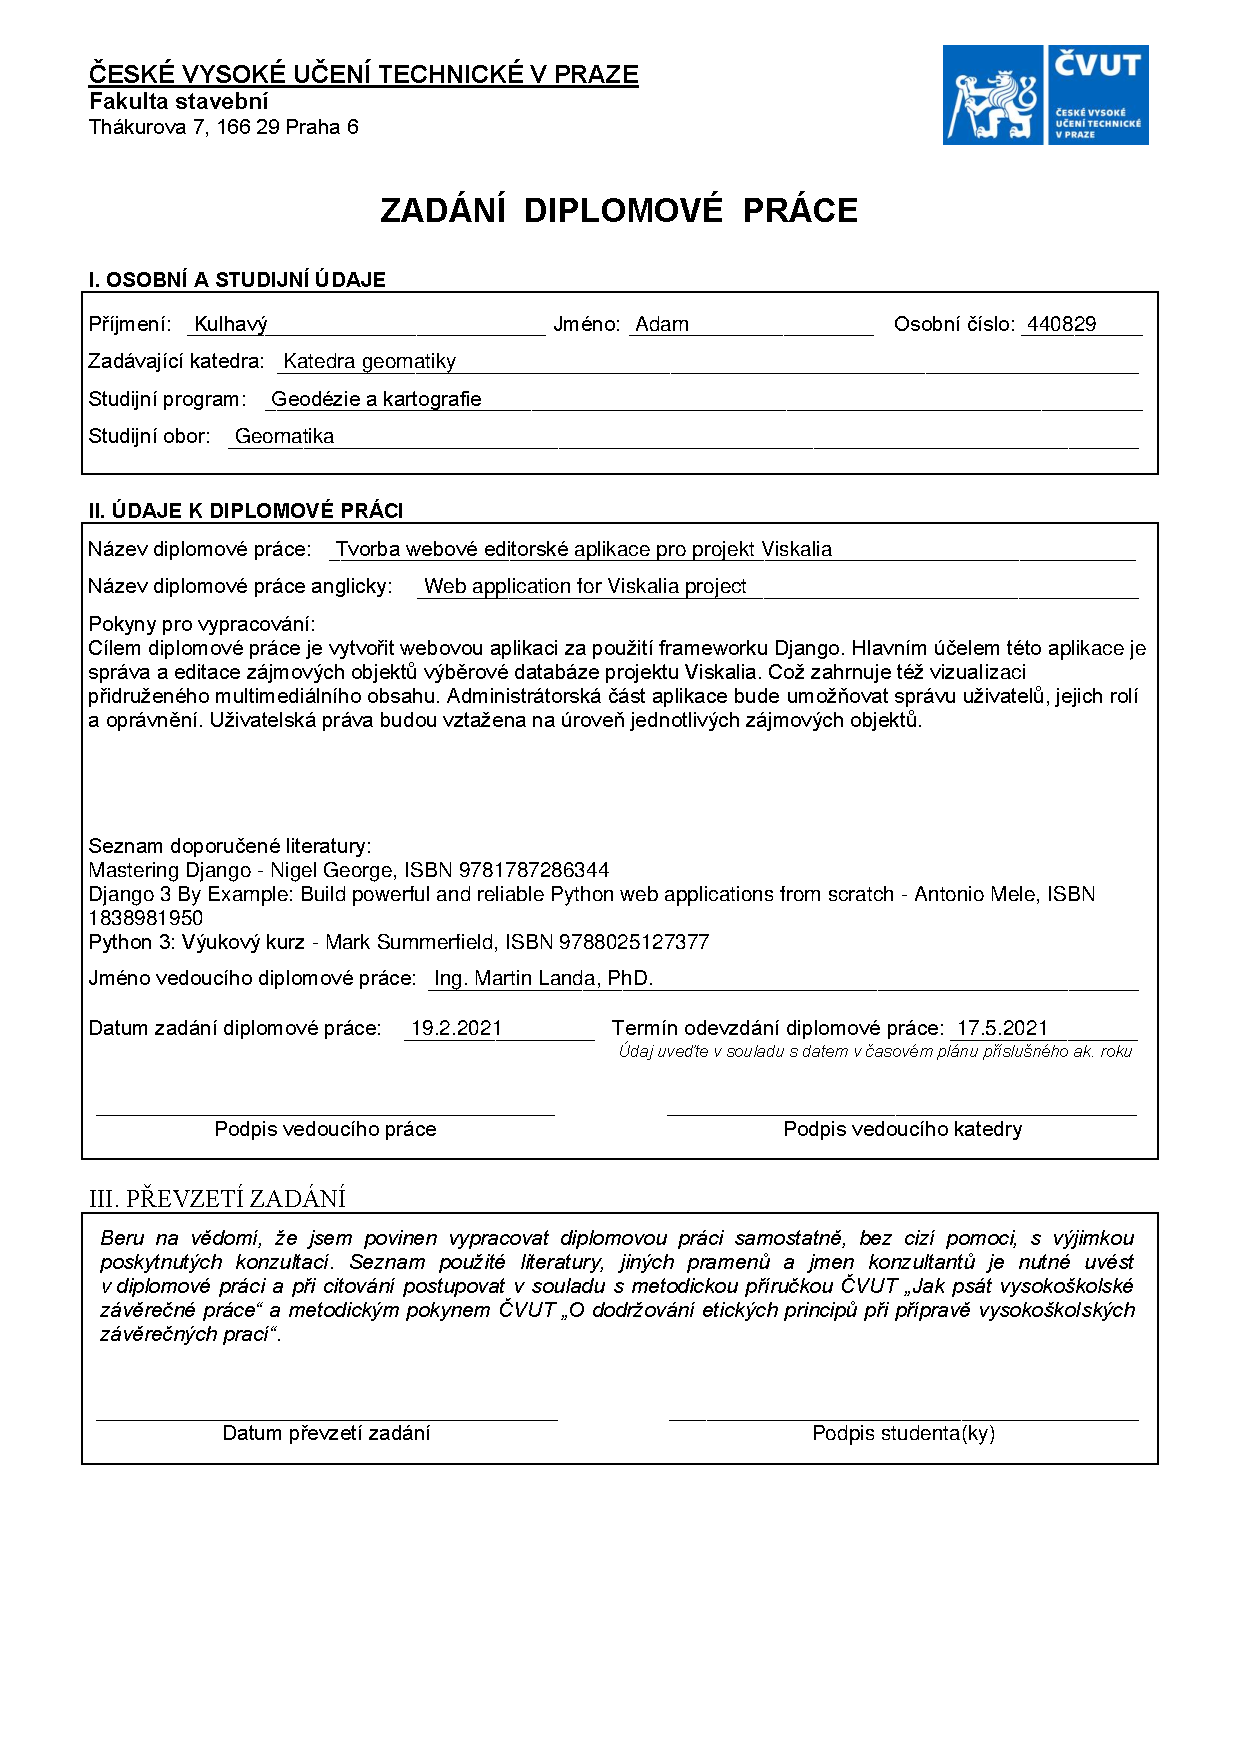
\includegraphics[scale=0.7]{../zadani/zadanidp.pdf}}%\sffamily\Huge\centering\ }%ZDE VLOŽIT LIST ZADÁNÍ}%
	%{\sffamily\centering Z~důvodu správného číslování stránek}

% Vysázení stránky s abstraktem
\vytvorabstrakt

% Vysázení prohlaseni o samostatnosti
\vytvorprohlaseni

% Vysázení poděkování
\stranka{%nahore
       }{%uprostred
       }{%dole
       \sffamily
	\begin{flushleft}
		\large
		\MakeUppercase{Poděkování}
	\end{flushleft}
	\vspace{1em}
		%\noindent
	\par\hspace{2ex}
	{Tímto bych rád poděkoval panu Ing. Martinu Landovi, Ph.D. za vedení diplomové práce a odbornou pomoc při jejím zpracování. Dále bych chtěl poděkovat celé své rodině za podporu a trpělivost.}
}

% Vysázení obsahu
\obsah

% Vysázení seznamu obrázků
\seznamobrazku

%% ML: vynechte, pokud nemate zadne tabulky
% Vysázení seznamu tabulek
%\seznamtabulek

% jednotlivé kapitoly
\chapter*{Úvod}
\addcontentsline{toc}{chapter}{Úvod}
\markboth{ÚVOD}{}
\label{0-uvod}

%% ML: stale jste neopravil sjednoceni casu, v textu se prolina
%% pritomny cas s budouci (dokonce v jedne kapitole!). Typicky se pise
%% v minulem case (z pohledu ctenare). Podstatne je ale zvolit stejny
%% cas v celem textu prace. Zvolte variantu tak, abyste nemusel
%% prepisovat cely text.

Cílem práce bylo vytvořit webovou aplikaci pro projekt VISKALIA
(Virtuální skansen lidové architektury), identifikační kód projektu:
DG20P02OVV003. Projekt se zaměřuje na záchranu fondů plánové, kresebné
a fotografické dokumentace lidové architektury v ČR. Jeho smyslem je
zpřístupnit tyto fondy širší veřejnosti. Toho se chce docílit
vytvořením virtuálního skansenu, který bude obsahovat zejména 3D
modely architektonických památek lidového stavitelství na území
ČR. Dále bude vytvořena veřejná databáze mapových výstupů, plánů,
fotografií a dalších dokumentů obohacená o množství metadat. Bude
využívána především při vzdělávání, ale také prostřednictvím výstav a
publikací.

Aplikace je zaměřená na interní správu objektů a nebude tedy přístupná
veřejnosti. Měla by umět zobrazovat data z databáze převzaté
z fondů Národního muzea. Ta bude dále rozšířena o uživateli poskytovaná
data jako fotografie, modely, dokumenty a jejich metadata. Tato data
už budou moci uživatelé přidávat, zobrazovat, mazat a editovat. Jeden
z hlavních požadavků je také na oprávnění k objektům, tedy aby
uživatelé mohli editovat pouze taková data, ke kterým mají udělené
oprávnění. Úkolem projektového týmu je také zajistit jednotný vývoj a nasazení 
aplikace společně s databází.

V první kapitole práce se diskutuje o možných technologických řešeních práce jako 
je volba vývojového prostředí aplikace nebo databázového systému. Na to navazují 
technologie, použité jak při vývoji aplikace, tak pro úpravu databázové struktury nebo 
automatického nasazení aplikace. Dále je popsáno navázání na rozpracovanou aplikaci a
použité databáze. Poslední kapitola se zabývá nejen samotným vývojem aplikace, ale také 
normalizací databáze a použitím softwaru Docker, pro vytvoření jednotného prostředí pro 
vývoj aplikace.




\chapter{Rešerše}
\label{1-reserse}

\section{Volba metody pro tvorbu webové aplikace}

Při volbě, jakou metodu pro tvorbu aplikace použít, se nabízelo několik
možností jak ji vytvořit. Aplikace by mohla být vytvořena například za použití
skriptovací jazyka \zk{PHP}, Javascriptu nebo Python frameworku 
pro tvorbu webových aplikací. 

Ze zadání projektového týmu ovšem vyplynulo, že by aplikace měla být
napsána v jazyce Python, a to z důvodu udržitelnosti kódu. Volba tedy
padla na Python frameworky.

\section{Volba Python frameworku}
Frameworkem je označována platforma, která se používá pro tvorbu aplikací. 
Je to soubor podpůrných programů a knihoven, které mají za cíl usnadnit 
jejich vývoj. Výběr vhodného frameworku byl vzhledem k jejich množství 
složitý. Mezi hlavní kritéria pro výběr frameworku se proto zařadila snadná
práce s databází, implementace oprávnění k objekům a dostupnost 
výukových materiálů a komunitní podpora. Díky těmto kritériím se nakonec 
vybíralo ze dvou frameworků, a to Flask a Django.

\begin{figure}[H] \centering
    
\includegraphics[width=240pt]{./pictures/1-django-vs-flask.jpeg}
    \caption[Flask vs Django]{Flask vs Django (\url{https://miro.medium.com/max/1672/1*TbMXbstb039keN-glx2CqQ.jpeg)}}
	\label{fig:Flask vs Django}                                
\end{figure}

Flask je open source webový framework napsaný v jazyce Python, klasifikovaný
jako mikro z důvodu, že není potřeba žádných dodatečných knihoven ani
jiných nástrojů. Do Flasku lze ovšem doinstalovat různá rozšíření,
která v základní verzi chybí jako například Flask-Admin, což je
administrátorské rozhraní pro správu uživatelů a objektů v
databázi. Výhodou je jeho velká obliba v komunitě, kdy v roce 2020 měl
druhé místo na github.com z webových frameworků, a díky tomu disponuje
spoustou materiálů a tutoriálů. Avšak velká nevýhoda Flasku pro vývoj
naší aplikace je, že nedisponuje datovými modely. Pokud bychom v průběhu
vývoje chtěli přidat sloupec do naší databáze, musíme to udělat ručně
v databázi a poté ho přidat do třídy ve webové aplikaci. \cite{flask}

Django je nejpoužívanějším open source frameworkem. Jednou z jeho funkcí je, že
disponuje objektově relačním mapováním. Jeho vlastností je tedy možnost generovat
model z databáze, který se zde může upravovat a poté jednoduchými
příkazy promítnout úpravy zpět do databáze. Další výhodou je implementované
administrátorské rozhraní a možnost doinstalováním přídavných balíčků,
poskytující jak grafické úpravy, tak přidané funkce. Jedním z nich je
i balíček django-guardian zajišťující podporu oprávnění k objektům. \cite{django}


Z těchto frameworků byl nakonec vybrán pro tvorbu aplikace framework
Django. Ten oproti Flasku disponoval snadnou a rychlou práci s modelem
databáze. Další výhodou je vývojáři implementované administrátorské
rozhraní, které se nemusí doinstalovat pomocí přídavného balíčku. Z
hlediska popularity a dostupnosti výuko\-vých materiálu jsou na tom oba
frameworky podobně, kdy se oba řadí na první dvě místa výrazně před
ostatní frameworky.

\vspace{10px}

\section{Volba databáze}

Jedním z hlavních úkolů bylo vytvoření databáze, ze které se budou
zobrazovat poskytnutá data z projektu \zk{Viskalia}, rozšířená o další
položky. Textová data zprostředkovaná fondem Národního muzea byla uložena v
MariaDB databázi a obrazová data byla v souborovém systému. Příslušná
databáze ovšem postrádá jakoukoli norma\-lizaci a data obsahují spoustu
duplicit. Nabízí se proto otázka, zda provést norma\-lizaci dat a opět
použít relační databázi, nebo nějakou z nerelačních
databází. Asi zásadní problém s \zk{NoSQL} databází, který by mohl nastat
je v komunikaci s frameworkem pro vývoj webových aplikací. Ty
v zásadě nemají problém komunikovat s jakýmkoliv typem relační
databáze, ovšem často nemají engine pro databáze typu \zk{NoSQL}. Byla 
tedy zvolena relační databáze a to MariaDB, z důvodu poskytnutí dat právě
z tohoto databázového systému. \cite{django} \cite{mariadb}

\newpage

\section{Automatizace nasazení aplikace}


Jedním z hlavních úkolů byla také automatizace nasazení aplikace a
zajištění bezpro\-blémového chodu na všech zařízeních. Při této otázce
se projektový tým nejprve musel rozhodnout, na jakém operačním systému se bude
aplikace vyvíjet a následně bude provozována. Po kratší úvaze se
zvolil systém Linux, který je vhodnější zejména pro vývoj aplikací v
jazyce Python. Zde se tedy hledal vhodný software pro
kontejnerizaci naší vyvíjené aplikace. Hlavními důvody pro jejich
použití je, že obsahují kompletní prostředí pro vývoj a chod aplikace
jako jsou knihovny nebo konfigurační soubory. Aplikace a všechny její
komponenty většinou běží v několika kontejnerech, které spolu dokáží
komunikovat. Jejich chod je od zbytku systému oddělen. Zde se nabízejí
dvě varianty, a to jsou \zk{LXC} (LinuX Containers) anebo Docker, což jsou
jedny z nejpoužívanějších aplikací. Hlavní rozdíl mezi těmito
aplikacemi je, že kontejnery \zk{LXC} obsahují svůj vlastní operační systém
a působí tedy spíše jako virtuální počítač. Docker oproti tomu žádné
takové prostředí nemá a běží pouze separovaně na operačním systému
uživatele. Dalším hlavním rozdílem je větší propracovanost Dockeru,
které umožňuje více nastavení kontejnerů a rozdělení aplikace do více
kontejnerů. Oproti \zk{LXC} může být Docker použit i na
jiném operačním systému než je Linux. Z těchto důvodů byl pro
kontejnerizaci zvolen Docker. \cite{deployment}

\newpage

\section{Normalizace databáze}

Normalizace databáze je reorganizace dat podle normalizačních standardů. 
Používá se pro snížení nadbytečných dat v databázi, například při duplicitách 
ve sloupcích. Normalizačních forem je pět, ale zpravidla se používají pouze 
první tři stupně. Jednotlivé stupně na sebe navzájem navazují, pokud budeme 
tedy chtít uplatnit třetí normalizační stupeň, musíme nejprve provést první a druhý.

První stupeň je v zásadě použití selského rozumu. Jedná se o odstranění 
dupli\-citních sloupců a sloupců, jež jsou kombinací jiných sloupců.

Druhý stupeň nám říká, že duplicitní hodnoty by měly být z tabulky odstraněny 
a přesunuty do nové tabulky, která je propojená cizím klíčem. Z tabulky se tedy 
odstraní všechny hodnoty, které platí pro více záznamů.

Třetí stupeň udává, že by tabulka neměla obsahovat hodnoty, které jsou na sobě závislé. 

Ve čtvrtém stupni by záznamy neměly obsahovat více nezávislých hodnot jedné podmnožiny. 
Takovéto hodnoty by opět měly být převedeny do samostatné tabulky a spojeny cizím klíčem.

Pátý stupeň platí, pokud není možné tabulku dále dělit bez ztráty dat. Po 
rozdělení by došlo ke ztrátě vztahů, které mezi daty platí. \cite{normalizace}



\section{Objektově relační mapování}

Objektově relační mapování (\zk{ORM}) zajišťuje konverzi dat mezi relační
databází a objektově orientovaným programovacím jazykem. Umožňuje
konverzi \zk{SQL} tabulek do tříd a usnadňuje tak práci s psaním \zk{SQL}
dotazů. Pro tuto konverzi se často používají externí programy, které
umožňují tyto konverze mezi řadou databázových systémů. Jedním z nich
je například SQLAlchemy, které umožňuje tuto konverzi pro programovací
jazyk Python a relační databáze SQLite, Postresql, MySQL a
další. Některé aplikace včetně Django si ovšem tuto konverzi
zprostředkovávají sami za pomoci vlastního \zk{ORM}. \cite{orm}
\cite{sqlalchemy}




















\chapter{Použité technologie}
\label{2-technologie}

\section{Django}

\begin{figure}[H] \centering
    
\includegraphics[width=160pt]{./pictures/django-logo.png}
    \caption[Django Logo]{Django Logo \cite{}}
	\label{fig:Django Logo}                                
\end{figure}

Django je open source prostředí, pro tvorbu webových aplikací. Django
je napsané v programovacím jazyku Python a pracuje na bázi
model-template-view. Model v tomto případě reprezentuje část, která je
schopna komunikovat a pracovat s databází. Templates určují obsah
zobrazení a jsou realizovány pomocí HTML. View zobrazuje daný obsah
koncovým uživatelům.

Django bylo vytvořeno v roce 2005 americkou společností The World
Company. Jeho první verze byla označena 0.90 a vyšla 16. listopadu
2005. Vývojáři pokračovali v jeho zdokonalování, kdy bylo během
následujících pár let provedeno několik aktualizací. V roce 2008 byla
vydána verze 1.0. Vývoj se nezastavil a po několika updatech byl v
roce 2013 vydána verze 1.5, která zajišťovala také podporu pro
Python 3, dříve pouze Python 2. Další velkou aktualizací bylo vydání nové
verze Django 2.0 na konci roku 2017. Ta zajišťovala plnou podporu pro
Python 3 a nadála už není možné pracovat s verzí Python 2. Aktuální
verze Djanga je 3.1, s tím že se plánuje v blízké době vydat verzi 3.2
po které by měl následovat další velká aktualizace v podobě Djanga 4.0,
která je plánována na začátek roku 2022.

\newpage


\subsection{Django - Instalace a inicializace projektu}

Django je framework pracující v jazyce Python, pro jehož aktuální
verzi 3.1 je potřeba mít nainstalován verzi Python 3.6 nebo
vyšší. Nejjednodušší je pomocí příkazové řádky spustit příkaz {\tt pip
install django}, čímž by se měla nainstalovat nejaktuálnější verze
Djanga. Po instalaci lze pro zobrazení aktuální verze použít příkaz
django-admin --version. Po instalaci se opět pomocí příkazové řádky
provede vytvoření projektu v aktuální složce příkazem {\tt django-admin
startproject [název projektu]}. Tímto se vytvoří nový adresář který
vypadá následovně:

\begin{itemize}
	\item \lbrack Název projektu\rbrack /
	\begin{itemize}
		\item manage.py
		\item \lbrack Název projektu\rbrack /
		\begin{itemize}
			\item \_\_init\_\_.py
			\item setting.py
			\item urls.py
			\item asgi.py
			\item wsgi.py
		\end{itemize}
	\end{itemize}
\end{itemize}

\vspace{6px}

\textbf{\_\_init\_\_.py} určuje, aby s adresářem bylo zacházeno jako s celkem.
\vspace{6px}

\textbf{setting.py} zde se definují všechna nastavení Django projektu. 
\vspace{6px}

\textbf{urls.py} v projektovém adresáři definuje seznam URL adres na
úrovní projektu. Při založení je zde obsažena administrátorská
stránka.  \vspace{6px}

\textbf{wsgi.py} (Web Server Gateway Interface) slouží pro propojení
webového serveru s frameworkem Django, popřípadě jinými webovými
aplikacemi.  \vspace{6px}

\textbf{asgi.py} (Asynchronous Server Gateway Interface) byl do Djanga
přidán ve verzi 3.0 a je nástupce staršího WSGI. Výhodou WSGI oproti
ASGI je, že dokáže pracovat se složitějšími protokoly jako jsou
WsbSocket, IoT protokoly, HTTP2 a další. Umožňuje komunikovat přes
více linek a tedy posílat a přijímat více dat najednou.  \vspace{6px}

\textbf{manage.py} je automaticky vygenerován v novém adresáři a je
přítomen v každém Django projektu. Je to nástroj pro spouštění
specifických příkazů například pro spuštění aplikace nebo vytvoření
aplikací.

\newpage

Pomocí nástroje manage.py se v Djangu spouští řada důležitých
příkazů. Zde je výčet těch nejdůležitějších a jejich popis.

\begin{itemize}
\item {\tt python manage.py runserver} - tento příkaz spouští
  aplikaci na lokálním serveru. Standardně je to na adrese
  127.0.0.1:8000. Aplikace je po spuštění přístupná pouze z daného
  zařízení a není možné se k ní připojit ani v rámci lokální
  sítě. Pokud je při spuštěném serveru provedena nějaká změna v kódu,
  framework projde celý projekt pro nalezení případné chyby a změna se
  automaticky zobrazí ve výstupu.
	
\item {\tt python manage.py makemigrations [název aplikace]} -
  tento příkaz provede porovnání modelu a s databází. Pokud jsou
  nalezeny změny, vytvoří se nový soubor se stávajícími migracemi. Ten
  obsahuje SQL příkazy, jak by se měla vytvořit databáze podle modelu
  definovaném v aplikaci. Příkaz se definuje zadáním jména aplikace,
  potažmo aplikací, lze tedy vytvořit migrace pouze pro jednu nebo
  více aplikací, zadáním jejich názvů.

\item {\tt python manage.py migrate} - spuštěním tohoto příkazu se
  synchronizuje databáze s modelem podle migračního souboru, který je
  generovaný z příkazu \newline {\tt makemigrations}.
	
\item {\tt python manage.py inspectdb} - příkaz vytvoří schéma
  připojené databáze a uloží ho do paměti. Vytvoření model.py souboru
  se pak provede spuštěním příkazu {\tt python manage.py inspectdb
    > models.py}.

\end{itemize}

\newpage

\subsection{Django - Tvorba aplikace}

Po založení projektu je potřeba vytvořit aplikaci. Počet použitých
aplikací v projektu není omezen a jejích výhodou je, že je lze
opětovně použít v dalších projektech. Aplikace se vytvoří příkazem{\tt
python manage.py startapp [nazev aplikace]}. Schéma je následující:

\begin{itemize}
	\item \lbrack Název aplikace\rbrack /
 	\begin{itemize}
 		\item \_\_init\_\_.py
		\item admin.py
		\item apps.py
		\item models.py
		\item urls.py
		\item \lbrack migrations\rbrack /
		\begin{itemize}
			\item \_\_init\_\_.py
		\end{itemize}
	\end{itemize}
\end{itemize}

\vspace{9px}

\textbf{\_\_init\_\_.py} má stejný význam jako v adresáři projektu. 
\vspace{6px}

\textbf{admin.py} slouží k registraci modelů do administrátorské
aplikace a k jejich úpravě.  \vspace{6px}

\textbf{apps.py} je konfigurační soubor, který obsahuje metadata o 
aplikaci.
\vspace{6px}

\textbf{models.py} obsahuje model databáze použitý v aplikaci.
\vspace{6px}

\textbf{urls.py} obsahuje všechny url adresy aplikace.
\vspace{6px}

\textbf{tests.py} obsahuje testovací metody, které se spustí při
testování funkčnosti aplikace.
\vspace{6px}

\textbf{migrations} ve složce migrations se nacházejí všechny migrační
soubory, vytvořené při spuštění příkazu \textit{makemigrations}

\newpage

\subsection{Django – práce s databází}


Další z věcí, kterou Django nabízí je jednoduchá a rychlá
práce s databází. Při práci s databází se používá soubor models.py,
který je při vytvoření projektu prázdný. Django standardně používá
databází SQLite, která se automaticky vytvoří v adresáři projektu. V
souboru settings.py lze ovšem nastavit připojení k vlastní, již
existující databázi. Při tvorbě databáze se do models.py tedy vytváří
modely jednotlivých tabulek, které poté pomocí příkazů makemigrations
a migrate vytvoří nebo upraví tabulky v naší databázi. S databází jako
takovou tedy vůbec nemusíme pracovat. Při připojování, k již
existující databázi lze příkazem inspectdb vygeneruje model stávající
databáze. Django oficiálně podporuje databáze PostgreSQL, MariaDB,
MySQL, Oracle a SQLite. Jsou zde ovšem i komunitně vytvořené balíčky
pro podporu NoSQL databáze MongoDB.

Model obsahuje všechny informace o tabulkách a jejich
sloupcích. Jednotlivé tabulky jsou v modelu vytvořeny jako třídy class
jmeno\_tabulky(models.Model). Každá třída pak obsahuje názvy
jednotlivých sloupců a jejich datové typy. V závorce jsou pak obsaženy
dodatečné informace jako například primární klíč, maximální délka
proměnné atd
\textit{first\_name=models.CharField(max\_length=30)}. Jednotlivé
třídy dále mohou obsahovat další třídy, například \textit{meta}, která obsahuje
dodatečné informace o tabulce.

\vspace{15px}

\begin{figure}[H] \centering
    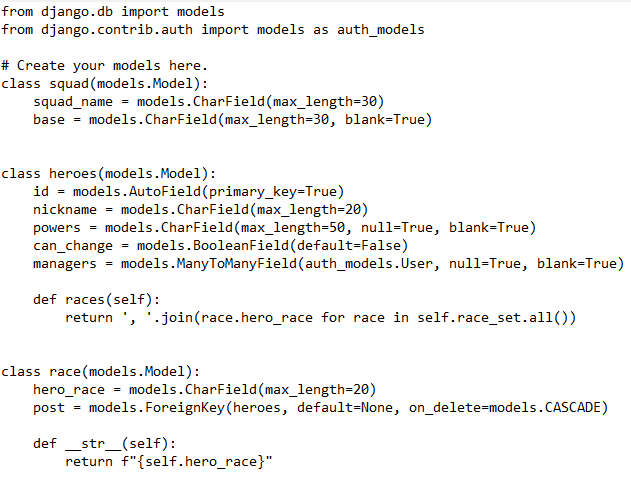
\includegraphics[width=300pt]{./pictures/2-model-example.png}
    \caption[Model příklad]{Ukázka models.py \cite{}}
	\label{fig:Ukázka models.py}                                
\end{figure}

\newpage

\subsection{Django - balíčky}

Packages, neboli balíčky jsou nástroje pro usnadnění práce s
djangem. Tyto balíčky mají mnoho funkcí, a to od změny vzhledu
stránky, až po implementaci nových funkcí do administrátorské aplikace. Většina
balíčků je tvořena komunitou a každý uživatel si také může vytvořit
svůj vlastní. Pro nalezení vhodného balíčku slouží například stránka
\textit{https://djangopackages.org}, kde lze najít všechna
rozšíření. Ty jsou zpravidla uloženy na stránce \textit{github.com}, kde
je detailně popsána jejich dokumentace. Jejich implementace je opravdu
jednoduchá, pomocí pip se nainstaluje příslušný balíček (např. {\tt pip
install django-rest)}. Dále se v projektu v souboru settings.py přidá
rozšíření do INSTALLED\_APPS a provede se migrace pro
vytvoření tabulek v databázi.

\subsection{Django - administrátorské rozhraní}

Jeden z nejdůležitějších komponentů Djanga je administrátorské
rozhraní, které dovoluje oprávněným uživatelům pracovat s daty
uloženými v databázi. Pomocí registrovaných modelů, může uživatel s
oprávněním prohlížet, přidávat, upravovat a mazat data v jednotlivých
modelech. Administrátorská aplikace je od té uživatelské oddělena a je
možné se do ní dostat přidáním \textit{/admin} za webovou adresu. Pro
přihlášení musí být uživatel registrován jako \textit{staff} a poté mu
musí být udělenu práva k jednotlivým modelům. V aplikaci je možné
nastavit práva jednotlivcům, popřípadě skupinám, do kterých se poté
uživatelé přidávají.

Registrace modelů a jejich následná úprava se prování v souboru
admin.py. Nejprve se modely musí importovat a poté registrovat pro
zobrazení v administrátorském rozhraní. Pokud je potřeba tabulky
modifikovat, například zobrazit jen některá data, je třeba vytvořit ke
každému modelu třídu, která se následně upravuje. Pro tento případ
Django disponuje velkou škálou funkcí pro jednoduchou úpravu zobrazení
dat.

\newpage

\section{Docker}

Docker je open source software používaný pro jednotný vývoj aplikací,
které běží v izolovaných kontejnerech. Je primárně využíván na
operačním systému Linux, ale je možné ho zprovoznit také na Windows
nebo Mac OS X. Výhodou je také, že může běžet jak lokálně, tak na
cloudovém uložišti. Jeho užití spočívá ve vytvoření obrazů (image), ze 
kterých se následně v kontejnerech spustí aplikace ve stejné formě, 
v jaké byl vytvořen její obraz. Díky tomu je poté zajištěn bezproblémový 
chod na jakémkoliv jiném zařízení se stejným operačním systémem. Image 
pro Linux může běžet pouze na systémech s Linux a stejně tak je to pro
Windows. Aplikace spuštěná v Dockeru je izolovaná, a nezasahuje do
ostatních aplikací. Je zde také snadná možnost testovat nové verze
knihoven a aplikací.

Při použití Dockeru je nutné nejprve vytvoří obraz, která obsahuje 
všechny aplikace a jejich nastavení potřebné pro bezproblémový chod. 
Z tohoto obrazu se poté vytvoří kontejner, který obsahuje také svou 
vlastní vrstvu, kde jsou uloženy všechny změny, které uživatel provedl.



\section{Git}

Git je open source verzovací systém, který se hojně používá při vývoji
aplikací. Jeho použití je možné na řadě platforem a ovládání
se provádí přes příkazový řádek nebo GUI. Git funguje na principu
repozitářů, ve kterých jsou uloženy projekty. Repozitář obsahuje celý
projekt a jeho kompletní historii provedených změn. Každý člen týmu je
tedy rovněž i zálohou. Při použití Gitu se využívají webové služby
jako například GitHub nebo GitLab, kde jsou repozitáře
zálohovány. Zároveň tu je mnoho užitečných nastavení jako veřejné nebo
soukromé repozitáře, nastavení práv uživatelů a spousta dalších.

\newpage

\section{MariaDB}

MariaDB je komunitně vyvíjeným databázovým systémem odvozeným od MySQL
licencovaný jako svobodný software GNU. První verze MariaDB vyšla v
roce 2009 a měla číslo 5.1, to odpovídalo aktuální verzi MySQL,
poslední verze této řady byla verze 5.5. Další řada nesla označení 10
a lišila se tím, že už nebyla 100\% kompatibilní s MySQL. Aktuálně
nejnovější verze je 10.5, která vyšla na konci roku 2019. MariaDB
podporuje řadu operačních systémů včetně těch nejrozšířenějších jako
Windows, Linux a MacOS. Vzhledem k tomu, že se vycházelo z MySQL, má
MariaDB stejnou strukturu a indexování. Oproti MySQL má ovšem daleko
rychlejší vývoj, což je způsobeno i tím, že je celý projekt open
source.

\section{phpMyAdmin}

Je to open source nástroj pro správu MySQL a MariaDB databáze pomocí
webového rozhraní. Je napsaný v jazyce PHP a je k dispozici v 80
jazycích včetně češtiny. Toto rozhraní umožňuje provádět SQL příkazy
jako jsou CREATE, DROP, ALTER table a spravovat obsah tabulek. Dále je
zde možno například import dat z CSV souborů, export dat do
nejrůznějších formátů nebo správa uživatelů. K přístupu do rozhraní
phpMyAdmin je zapotřebí webový prohlížeč s podporou cookies a
JavaScriptu.

\section{Objektově relační mapování}

Objektově relační mapování (ORM) zajišťuje konverzi dat mezi relační databází a objektově orientovaným programovacím jazykem. Umožňuje konverzi SQL tabulek do tříd a usnadňuje tak práci s psaním SQL dotazů. Pro tuto konverzi se často používají externí programy, které umožňují tyto konverze mezi řadou databázových systémů. Jedním z nich je například SQLAlchemy, které umožňuje tuto konverzi pro programovací jazyk Python a databáze SQLite, Postresql, MySQL a další. Některé aplikace včetně Django si ovšem tuto konverzi zprostředkovávají sami za pomoci vlastního ORM. 

\textbf{}
\textit{}





\chapter{Seznámení s aplikací a databází}
\label{3-seznameni-s-aplikaci-a-databazi}

\section{Navázání na projekt FGIS}

Tato diplomová práce navazuje na započatý projekt z předmětu Free
Software GIS. Na projektu se také podílel autor práce. 
Projekt měl za úkol vytvořit jednoduchou webovou aplikaci, kdy
přihlášení uživatelé mohli zobrazovat, vytvářet, editovat a mazat záznamy
z databáze. Databáze pro tento projekt byla pouze cvičná a obsahovala
pouze několik tabulek s textovými poli. Projekt ovšem nebyl zcela
dokončen, protože se nepovedlo vytvořit všechny funkce tak, aby
správně fungovali. Data do databáze šla přidávat, zobrazovat je a 
mazat, ale při editaci se po uložení nepřepsala aktuální data v
databázi.

\begin{figure}[H] \centering
    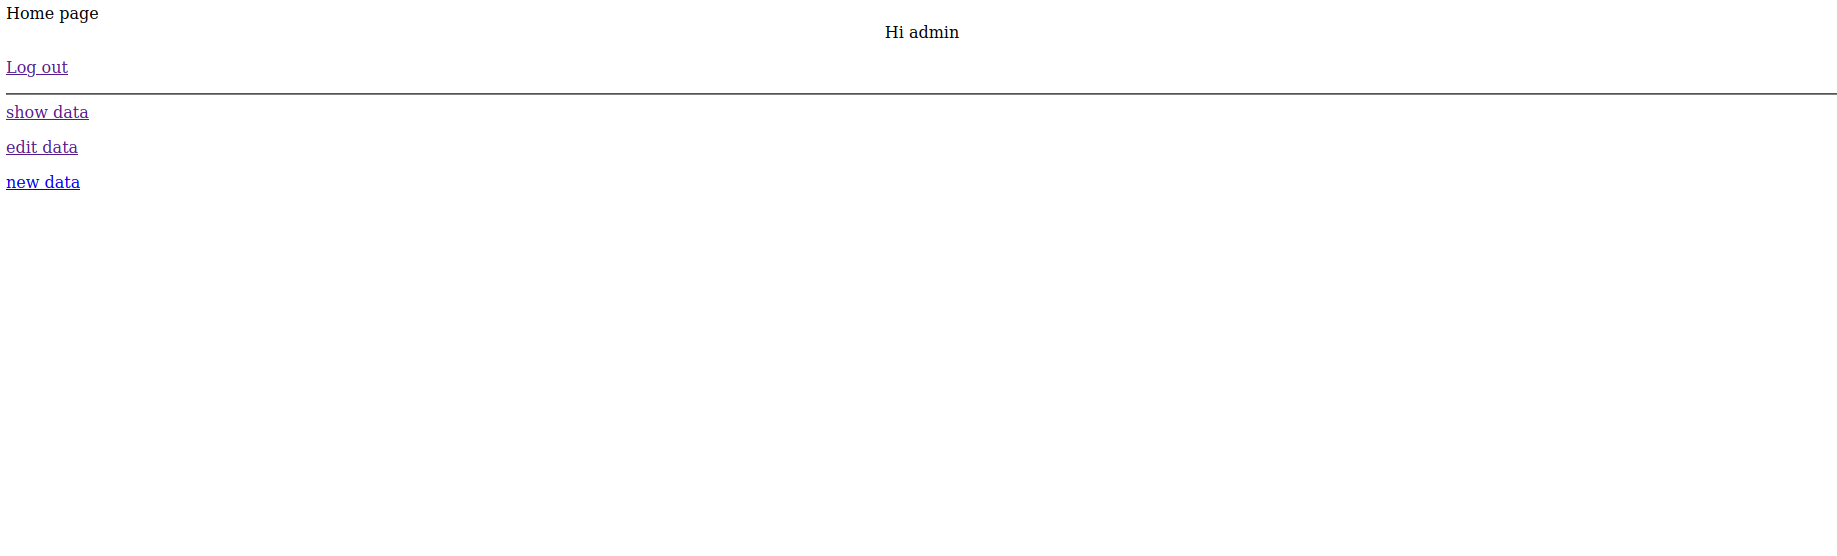
\includegraphics[width=400pt]{./pictures/4-nahled-menu-fgis.PNG}
    \caption[Náhled aplikace vytvořené v projektu FGIS]{Náhled aplikace vytvořené v projektu FGIS}
	\label{fig:Náhled aplikace}              
\end{figure}
 
 \section{Zkušební databáze}
 
Na začátku projektu byla používána pouze zkušební databáze, jejíž použití 
bylo z důvodu neznalosti přesné struktury finální databáze. Zkušební databáze 
sloužila na začátku projektu pro inicializaci aplikace, a vytvoření základních 
funkcionalit. Databáze obsahovala pouze tabulku s textovými daty.

 \newpage

\section{Centrální databáze}

Databáze fondů Národního muzea obsahuje objekty, které se budou ve 
vyvíjené aplikaci zobrazovat a budou rozšířena o další data. Všechna data 
v této databázi jsou obsažena v jedná tabulace. Část sloupců v této tabulce 
obsahuje informace o objektu a část o obrázku, který je k němu přidělen. 
Jednotlivé objekty ovšem disponují více obrázky, kdy se pro každý obrázek
%% ML: objekt -> zaznam
vytváří nový databázový objekt. Zde dochází k duplikování velké části dat, 
kdy se sloupce s informacemi o objektu kopírují a mění se pouze část s 
obrázky a jejich metadaty. Databáze je tedy v nenormalizované formě.

\begin{figure}[H] \centering
    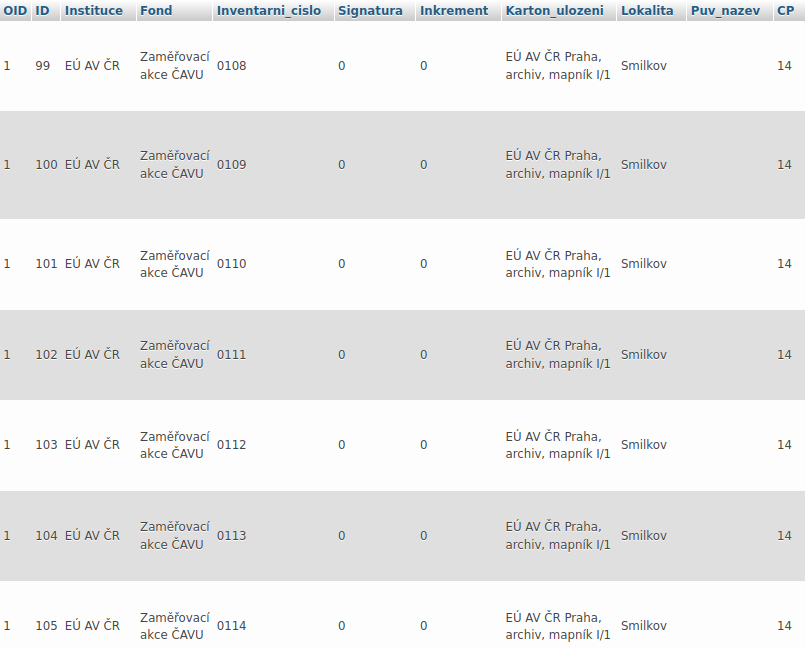
\includegraphics[width=420pt]{./pictures/5-ukazka-basedata.PNG}
    \caption[Náhled dat z centrální databáze s viditelnými duplicitami]{Náhled dat centrální z databáze s viditelnými duplicitami}
	\label{fig:Náhled dat z centrální databáze s viditelnými duplicitami}              
\end{figure}



\chapter{Tvorba aplikace}
\label{4-tvorba-aplikace}

\section{Vytvoření základní aplikace}

Aplikace, která byla vytvořena v projektu FGIS nebyla vytvořena správně, a obsahovala zbytečně složitý, a chybný kód. Začalo se tedy od začátku. Nejprve byla vytvořen projekt příkazem \emph{django-admin startproject mysite}. V projektu následně byla vytvořena aplikace pomocí \emph{python manage.py startapp}. Aplikace byla v \emph{settings.py} přidána do \textbf{INSTALLED\_APPS}. Dále se nastavilo připojení k databázi. V \emph{settings.py} se tedy v \textbf{DATABASES} se změnil engine na MySQL, protože Django v základu používá SQLite. Změnilo se ještě NAME, USER, PASSWORD, HOST A PORT, protože databáze byla provozována na školním serveru geo102.fsv.cvut.cz. Po připojení se musel vygenerovat model databáze, příkazem inspectdb, viz. Instalace a inicializace projektu. Dále byla provedena migrace, aby se v databázi vytvořily Django tabulky. Posledním krokem bylo vytvoření superuživatele, který se bude moci přihlásit do naší i administrátorské aplikace. To bylo realizováno příkazem \emph{python manage.py createsuperuser}.

Na stránce GitLab byl vytvořen nový repozitář, do kterého se celý projekt přesunul a nadále v něm byl průběžně zálohován. Dále se tam vytvářely tzv. \emph{issues}, kde se plánovaly nadcházející úkoly při tvorbě aplikace.

\section{Tvorba aplikace v uživatelském prostředí}

Prvním větším úkolem bylo vytvořit aplikace, která bude zobrazovat data, a po přihlášení je bude moci uživatel také přidávat, mazat a editovat. Nejprve se tady do adresáře aplikace přidala soubor urls.py, který se následně připojil do projektového adresáře urls.py. Tento způsob je výhodný při použití více aplikace, kdy si každá aplikace uchovává své url adresy a projekt je tak přehlednější. Pokračovalo se vytvořením pohledů založených na třídách, které se v Pythonu používají pro nahrazení pohledů jako funkcí. Použity jsou základní pohledy jako ListView pro zobrazení obsahu tabulky nebo CreateView pro uložení dat do databáze. V aplikaci v soubory \emph{views.py} jsou tedy vytvořeny třídy pohledů pro každou url adresu. Definice těchto tříd vypadá následovně \emph{class “název třídy“(Listview):} dále se u třídy definuje model, který se má zobrazit a template\_name neboli název šablony, která se použije při zobrazení.

\begin{figure}[H] \centering
    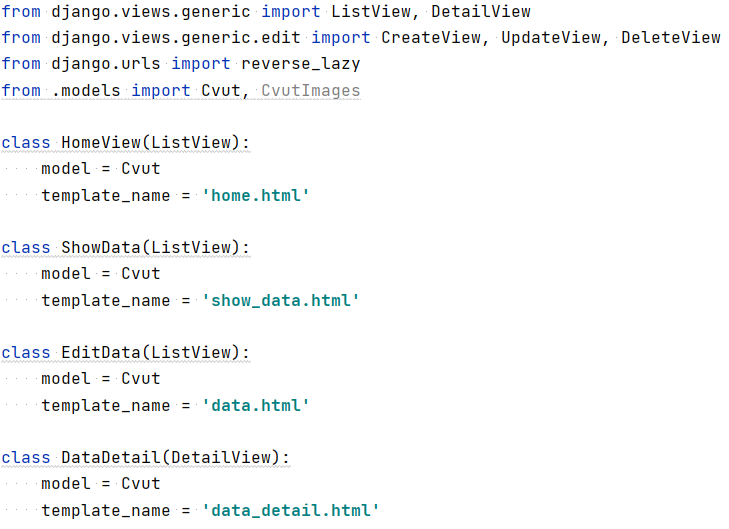
\includegraphics[width=350pt]{./pictures/6-nahled-views-aplikace.PNG}
    \caption[Náhled views.py a jeho tříd]{Náhled views.py a jeho tříd}
	\label{fig:Náhled views.py a jeho tříd}              
\end{figure}


V souboru \emph{urls.py} jsou propojeny url adresy, pohledy a html šablony, na které se odkazují. Do urls.py musí být zároveň importovány všechny použité pohledy. Dále se provede import \emph{path}. Poté se sestaví \emph{urlpatterns}, což je seznam, který obsahuje jednotlivé adresy. Ty jsou v něm uvedeny ve funkci path, která má dva povinné argumenty, route a view a dva nepovinné, name a kwargs. Route uvádí adresu, pod jakou se bude stránka načítat a view odkazuje na importovaný pohled. Zde byla použita funkce \emph{as\_view()}, která se používá, pokud je pohled typu třída. Jméno je uvedeno jako název html šablony.

\begin{figure}[H] \centering
    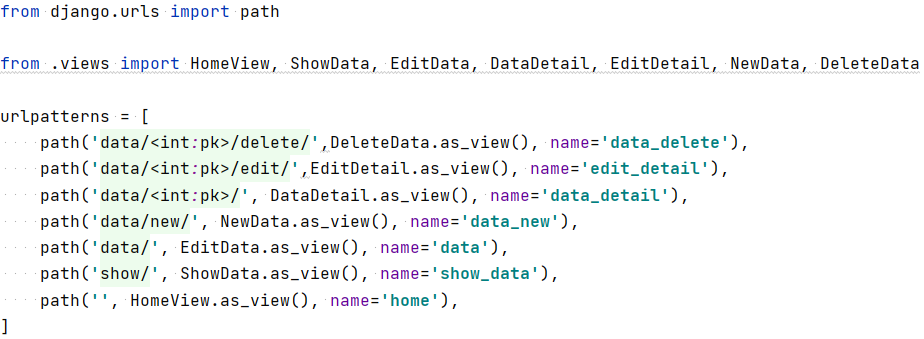
\includegraphics[width=450pt]{./pictures/7-urls-aplikace.PNG}
    \caption[Náhled urls.py v adresáři aplikaci]{Náhled urls.py v adresáři aplikaci}
	\label{fig:Náhled urls.py v adresáři aplikaci}              
\end{figure}

Pro vytvoření html šablon se vytvořila složka \emph{templates}, kde jsou uloženy jednotlivé html soubory. Tato složka se v settings.py nastaví jako výchozí pro jejich zobrazení. Poté se už mohou vytvářet jednotlivé šablony. Šablony jsou vždy vytvořeny s podmínkou \emph{if user.is\_authenticated}, tedy pokud je uživatel přihlášen, zobrazí se mu na stránce možnosti data editovat, vytvářet a mazat. S tímto je spojena ještě další změna v \emph{settings.py}, kde je přidáno \textbf{LOGIN\_REDIRECT\_URL = 'home'} a \textbf{LOGOUT\_REDIRECT\_URL = 'home'} které uživatele po přihlášení a odhlášení přesměruje na domovskou stránku. Ve složce \emph{templates} je ještě složka \emph{registration}, kde je umístěn \emph{login.html}. Html soubory zobrazují data v základní formě tabulek a nejsou graficky upravována pomocí css. 

\begin{figure}[H] \centering
    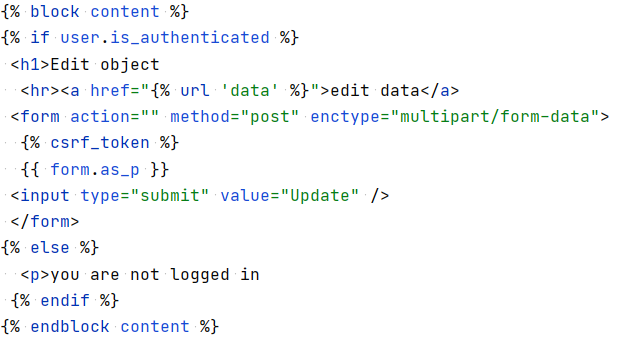
\includegraphics[width=350pt]{./pictures/8-edit-detail-html.PNG}
    \caption[Náhled html souboru edit detail]{Náhled html souboru edit detail}
	\label{fig:Náhled html souboru edit detail}
\end{figure}


\newpage

\section{Přidání obrázků}

Dalším úkolem bylo vyřešit přidávání obrázků k jednotlivým záznamům. Obrázky by se neměly ukládat do databáze, ale do adresáře v aplikaci. Databáze poté bude obsahovat cestu k těmto souborům. K tomu byla vytvořena nová tabulka, který byla přes cizí klíč spojena s tabulkou se záznamy. Tabulka byla vytvořena v modelu, a poté pomocí migrací byl přenesena do databáze. Obsahuje tedy pole ID, což je primární klíč tabulky, Post, který je cizím klíčem k tabulce Cvut a sloupec Image, do kterého se zaznamenává cesta k danému souboru.

\begin{figure}[H] \centering
    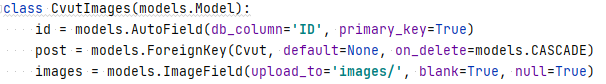
\includegraphics[width=430pt]{./pictures/9-db-cvutimages.PNG}
    \caption[Náhled tabulky CvutImages pro ukládání obrázků]{Náhled tabulky CvutImages pro ukládání obrázk}
	\label{fig:Náhled tabulky CvutImages pro ukládání obrázk}              
\end{figure}

V nastavení se dále určí rootovský adresář pro nahrávané soubory \textbf{MEDIA\_ROOT = os.path.join(BASE\_DIR, 'media')} a \textbf{MEDIA\_URL = '/media/'}.
A v poslední řadě se musí nastavit v projektovém urls.py media soubory, které django samo neumí zobrazovat. Zde se provede import settings a static a k urlpatterns se připojí funkce static. 

\begin{figure}[H] \centering
    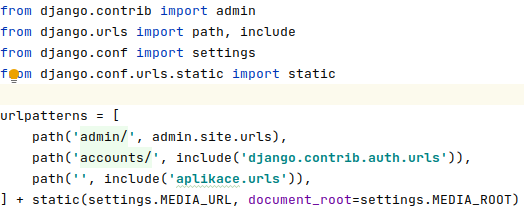
\includegraphics[width=350pt]{./pictures/10-media-urlspy.PNG}
    \caption[Náhled projektového urls.py]{Náhled projektového urls.py}
	\label{fig:Náhled projektového urls.py}              
\end{figure}

\newpage

\section{Statické soubory}

Pro řešení vizuální stránky webu jsou používány css soubory. Ve složce aplikace se tedy vytvoří adresář static a tomu v \emph{settings} se určí jeho nastavení pro statické soubory příkazy \textbf{STATIC\_URL = '/static/'} a \textbf{STATICFILES\_DIRS = [os.path.join(BASE\_DIR, 'static')]}. Ve složce static je vytvořen adresář css, kde se nachází základní css soubor base.css. Ten je ovšem prázdný a není připojen k žádnému html souboru.

\section{Nastavení jazyka a času}

Dalším nastavením bylo použití našeho středoevropského času a českého jazyka. Velice jednoduché nastavení, kdy v \emph{settings} je po vytvoření aplikace nastaven jazyk na angličtinu a čas na UTC. Pro změnu se tedy přepíše \textbf{LANGUAGE\_CODE = 'en-us'} na \textbf{LANGUAGE\_CODE = 'cs'} a \textbf{TIME\_ZONE = 'UTC'} na \textbf{TIME\_ZONE = 'CET'}.























\chapter*{Závěr}
\label{5-zaver}
\addcontentsline{toc}{chapter}{Závěr}

Cílem práce bylo vytvořit webovou aplikaci pro projekt
\zk{Viskalia}. Aplikace měla být vytvořena tak, aby uměla zobrazovat,
vytvářet, editovat a mazat data v databázi. Tento základní předpoklad
byl splněn, kdy aplikace splňuje všechny tyto funkcion\-ality i s
náležitými úpravami.

Co se týče aplikace, je zde několik možností na zlepšení, popřípadě
dodělání nedostatků aplikace. Jedním z nedostatků je pracná tvorba
vytváření uživatelů a nastavování jejich práv k objektům, kdy se
každému uživateli musí samostatně nastavit práva ke každému objektu,
pro který by měl mít právo editace. Toto by šlo vyřešit jednoduchým
skriptem pro hromadný zápis práv do tabulky Managers. Dalším
nedostatkem je použití balíčku pro editaci administrátorského
prostředí \emph{admin\_interface}. Aktuálním problémem je chybějící šablona, která
by se při se\-stavování kontejnerů vložila do databáze. Při opětovném
vytvoření se tedy vždy restartuje nastavení, které superuživatel
vytvoří. Možným řešením je tuto šablonu vytvořit a přidat jí při
spouštění do tabulky \emph{admin\_interface}, nebo toto rozšíření odstranit a
upravit základní \zk{HTML} šablonu, kterou poskytuje Django. Posledním
námětem je dokončení uživatelské aplikace, aby byla uživatelsky
přívětivější, ať už se jedná pouze o zobrazování dat, nebo dodělání
funkcionalit podobných admi\-nistrátorskému rozhraní.

Jedním z úkolů projektového týmu \zk{Viskalia} bylo také automatizovat
nasazení aplikace a databáze. Tento problém byl také vyřešen, ovšem
obsahuje několik nedostatků, které by bylo potřeba opravit. Prvním
nedostatkem je synchronizace struktury databáze a vložených dat, kdy
při tvorbě tabulky, která přebírá data z centrální databáze není
proveden sken této databáze, ale je přímo vytvořena tabulka, která
odpovídá její aktuální verzi. Pokud se tedy provedou změny v této
databázi, nepromítnou se do námi vytvořená tabulky. Dalším problémem
je stahování obrázků z databázového serveru. Obrázky nejsou stahovány
z databázového serveru, ale je stahován pouze předpřipravený soubor s
několika vybranými obrázky.


% Vysázení seznamu zkratek
\begin{seznamzkratek}{ABCDE}      

      \novazkratka{Viskalia}
          {Viskalia}
          {Virtuální skansen lidové architektury} 

      \novazkratka{SQL}
          {SQL}
          {Standardizovaný strukturovaný dotazovací jazyk (Structured Query Language)} 

      \novazkratka{NoSQL}
          {NoSQL}
          {Ne jenom SQL (Not only SQL)} 

      \novazkratka{PHP}
	{PHP}
	{Hypertextový preprocesor (Hypertext Preprocessor)}

      \novazkratka{LXC}
	{LXC}
	{Linuxové Kontejnery (LinuX Containers)}

      \novazkratka{HTML}	
	{HTML}
	{Hypertextový značkovací jazyk (Hypertext Markup Language)}  
	             	                   
      \novazkratka{CSS}
          {CSS}
          {Kaskádové styly (Cascading Style Sheets)} 
          
      \novazkratka{ORM}
	{ORM}
	{Objektově relační zobrazení (Object-relational mapping)}
            
      \novazkratka{ID}	
	{ID}
	{Hodnota jednoznačně určující každý záznam} 	      	     
          
      \novazkratka{URL}
          {URL}
          {Jednotná adresa zdroje (Uniform Resource Locator)}                
          
      \novazkratka{WSGI}
	{WSGI}
	{Web Server Gateway Interface}
                                          
      \novazkratka{ASGI}
          {ASGI}
          {Asynchronous Server Gateway Interface} 	
          
      \novazkratka{HTTP2}
          {HTTP2}
          {Hypertext Transfer Protocol 2} 	

      \novazkratka{IoT}
          {IoT}
          {Internet věcí (Internet of Things)} 	

      \novazkratka{OS}
          {OS}
          {Operační systém (Operating system)} 	

      \novazkratka{GUI}
          {GUI}
          {Grafické uživatelské rozhranít (Graphic User Interface)} 	

      \novazkratka{CSV}
          {CSV}
          {Hodnoty oddělené čárkami (Comma-separated values)} 	

      \novazkratka{GIS}
          {GIS}
          {Geografický informační systém (Geographic information system)} 	

      \novazkratka{FGIS}
          {FGIS}
          {Free software GIS} 	

      \novazkratka{UTC}
          {UTC}
          {Koordinovaný světový čas (Coordinated Universal Time)} 

	
     	      
\end{seznamzkratek}

% Literatura
\nocite{*}
\def\refname{Odkazy}
\bibliographystyle{unsrt}
\bibliography{literatura}


% Začátek příloh
\def\figurename{Figure}%
\prilohy

% Vysázení seznamu příloh
\seznampriloh

%% Vložení souboru s přílohami
\chapter{Průvodce aplikací}
\label{Průvodce aplikací}


Po zadání webové adresy do administrátorského rozhraní se zobrazí přihlašovací okno. Pro úspěšné přihlášení musí být uživatel nastaven jako staff. 

\begin{figure}[H] \centering
  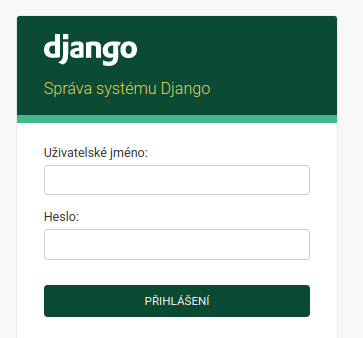
\includegraphics[width=200pt]{./pictures/50-prihlaseni.png}
    \caption[Přihlašování do administrátorské aplikace]{Přihlašování do administrátorské aplikace}
	\label{Přihlašování do administrátorské aplikace}                                
\end{figure}


Pokud se uživatel přihlásí jako administrátor (superuser), má přístup ke všem funkcím a tabulkám, které Django poskytuje. To je editování vzhledu stránky, přidávání, editování a mazání uživatelů a skupin a přístup do tabulky Cvut s přidruženými tabulkami.

\begin{figure}[H] \centering
  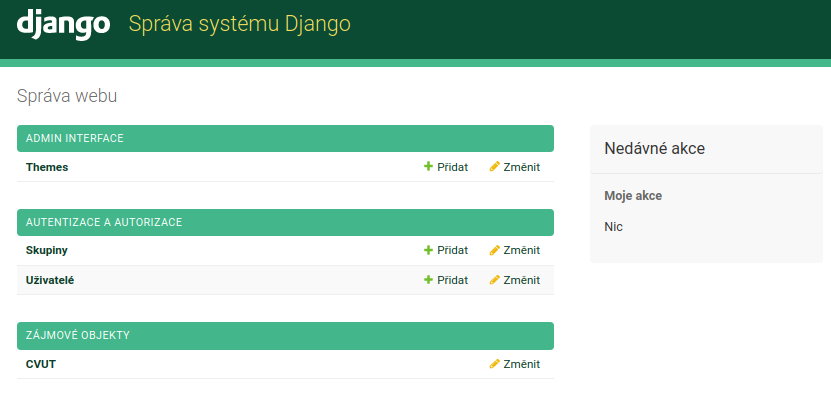
\includegraphics[width=420pt]{./pictures/51-mp-admin.png}
    \caption[Hlavní stránka pro přihlášení jako administrátor]{Hlavní stránka pro přihlášení jako administrátor}
	\label{Hlavní stránka pro přihlášení jako administrátor}                                
\end{figure}

\newpage

Zobrazení stránky pro uživatele, který má přístup pouze k tabulce Cvut.

\begin{figure}[H] \centering
  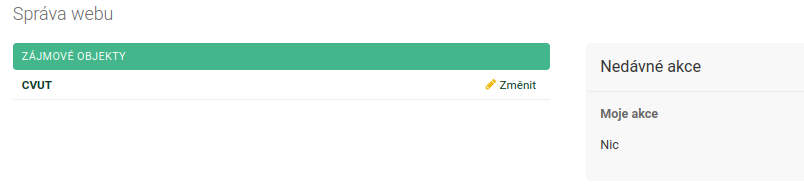
\includegraphics[width=320pt]{./pictures/58-uzivatel.png}
    \caption[Zobrazení stránky pro uživatele]{Zobrazení stránky pro uživatele}
	\label{Zobrazení stránky pro uživatele}                                
\end{figure}

Zobrazení tabulky Cvut s filtry a vyhledáváním.

\begin{figure}[H] \centering
  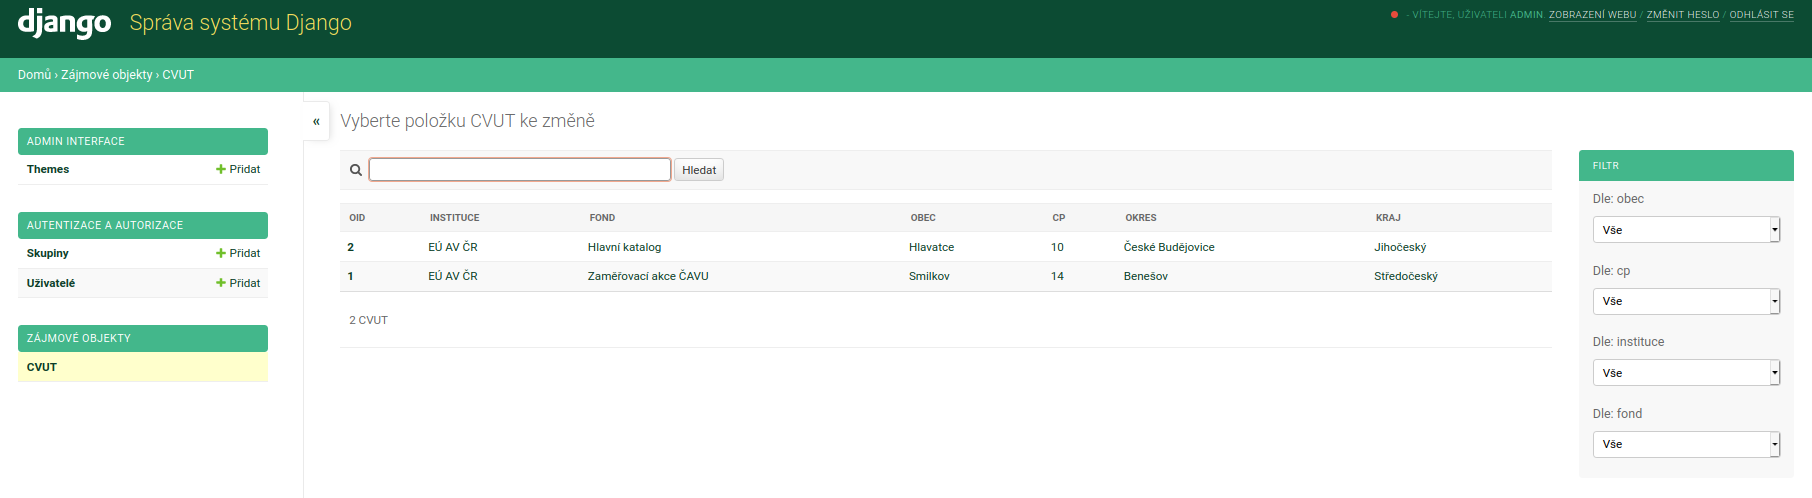
\includegraphics[width=420pt]{./pictures/52-cvut-admin.png}
    \caption[Hlavní stránka pro přihlášení jako administrátor]{Hlavní stránka pro přihlášení jako administrátor}
	\label{Hlavní stránka pro přihlášení jako administrátor}                                
\end{figure}


Po rozkliknutí záznamu se o něm zobrazí všechan data z tabulek Cvut, Base\_Images a CvutFiles. Superuživatelé mají možnost měnit práva k objektům pomocí tabulky Managers.

\begin{figure}[H] \centering
  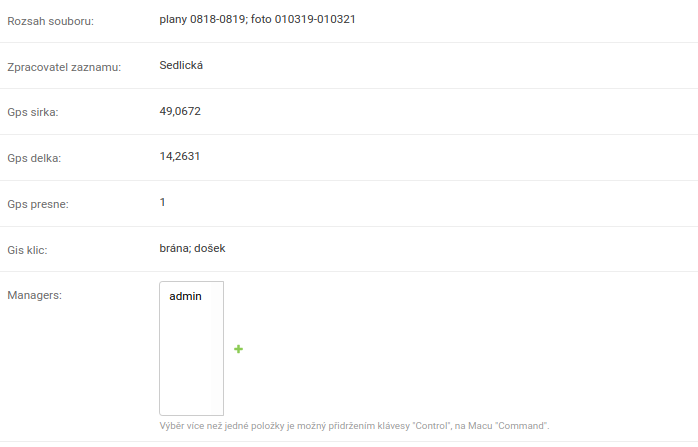
\includegraphics[width=340pt]{./pictures/53-data-managers.png}
    \caption[Zobrazení záznamu s možností měnit práva uživatelů]{Zobrazení záznamu s možností měnit práva uživatelů}
	\label{Zobrazení záznamu s možností měnit práva uživatelů}                                
\end{figure}


Zobrazení fotografií s náhledem z tabulky Base\_Images a souborů z tabulky CvutFiles. Možnost přidání a editace soubrů je možná, jen pokud k tomu má uživatel oprávnění.

\begin{figure}[H] \centering
  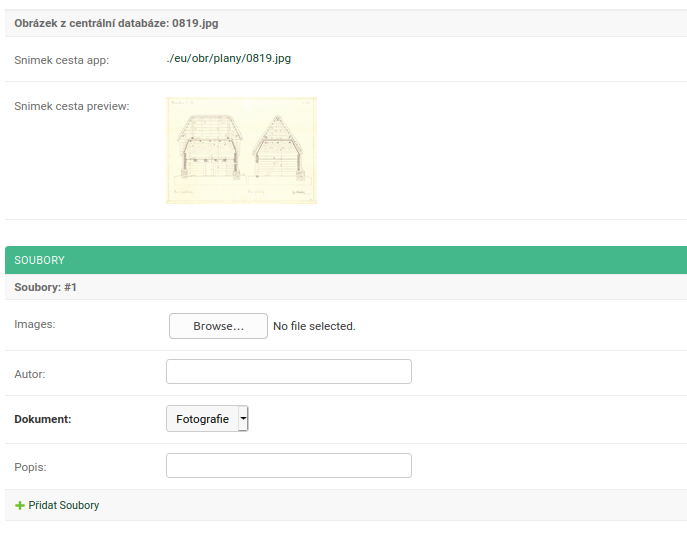
\includegraphics[width=320pt]{./pictures/54-obrazky.png}
    \caption[Zobrazení záznamu s možností měnit práva uživatelů]{Zobrazení záznamu s možností měnit práva uživatelů}
	\label{Zobrazení záznamu s možností měnit práva uživatelů}                                
\end{figure}


Po rozkliknutí \emph{Uživatelé} se zobrazí seznam všech uživatelů. Zde je možnost jejich editace, kde lze nastavit administrátorský přístup, superuživatele, zařadit uživatele do skupin nebo mu přiřadit jednotlivá práva.

\begin{figure}[H] \centering
  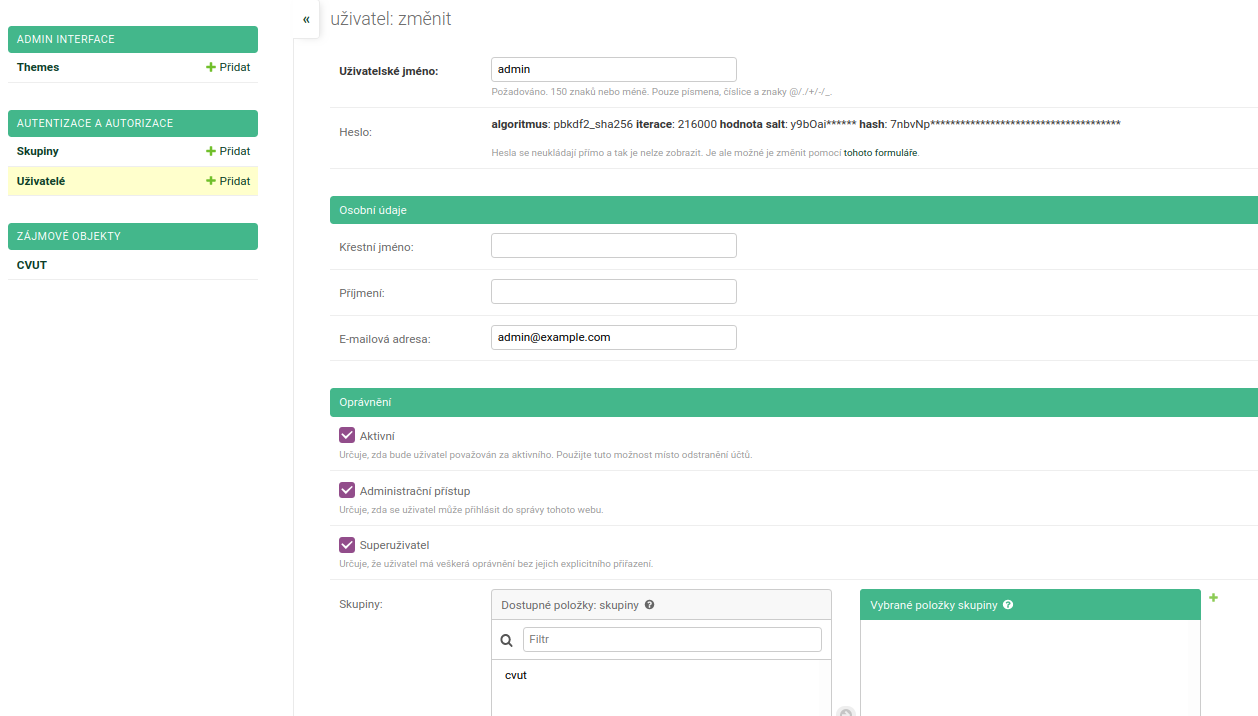
\includegraphics[width=390pt]{./pictures/55-sprava-uzivatelu.png}
    \caption[Správa uživatelů]{Správa uživatelů}
	\label{Správa uživatelů}                                
\end{figure}


Možnost nastavení skupin, u kterých lze navolit jednotlivá práva a poté do nich jednoduše přidávat uživatele.

\begin{figure}[H] \centering
  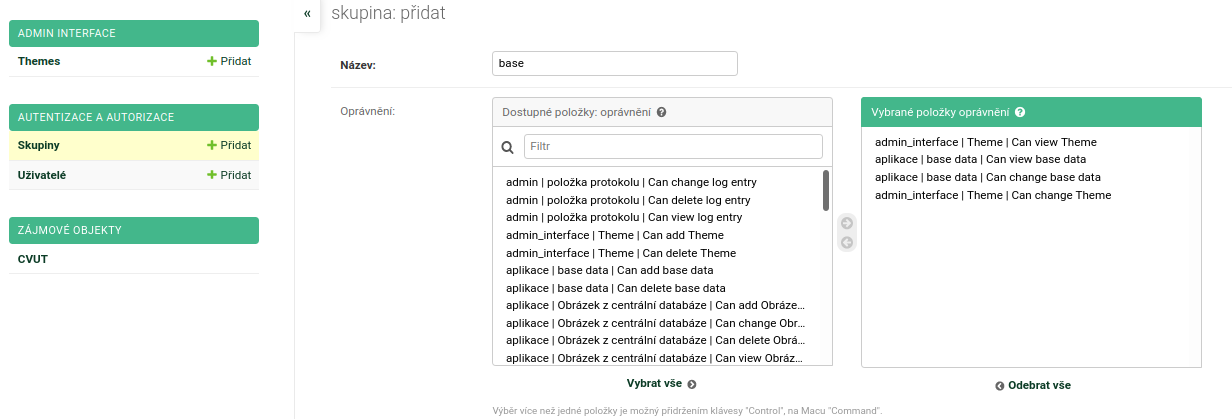
\includegraphics[width=420pt]{./pictures/56-skupiny.png}
    \caption[Tvorba skupin]{Tvorba skupin}
	\label{Tvorba skupin}                                
\end{figure}


V nastavení \emph{Theme} se může jednoduše měnit styl zobrazení stránky. Nastavit se dá například logo stránky, barva pozadí nebo textu.

\begin{figure}[H] \centering
  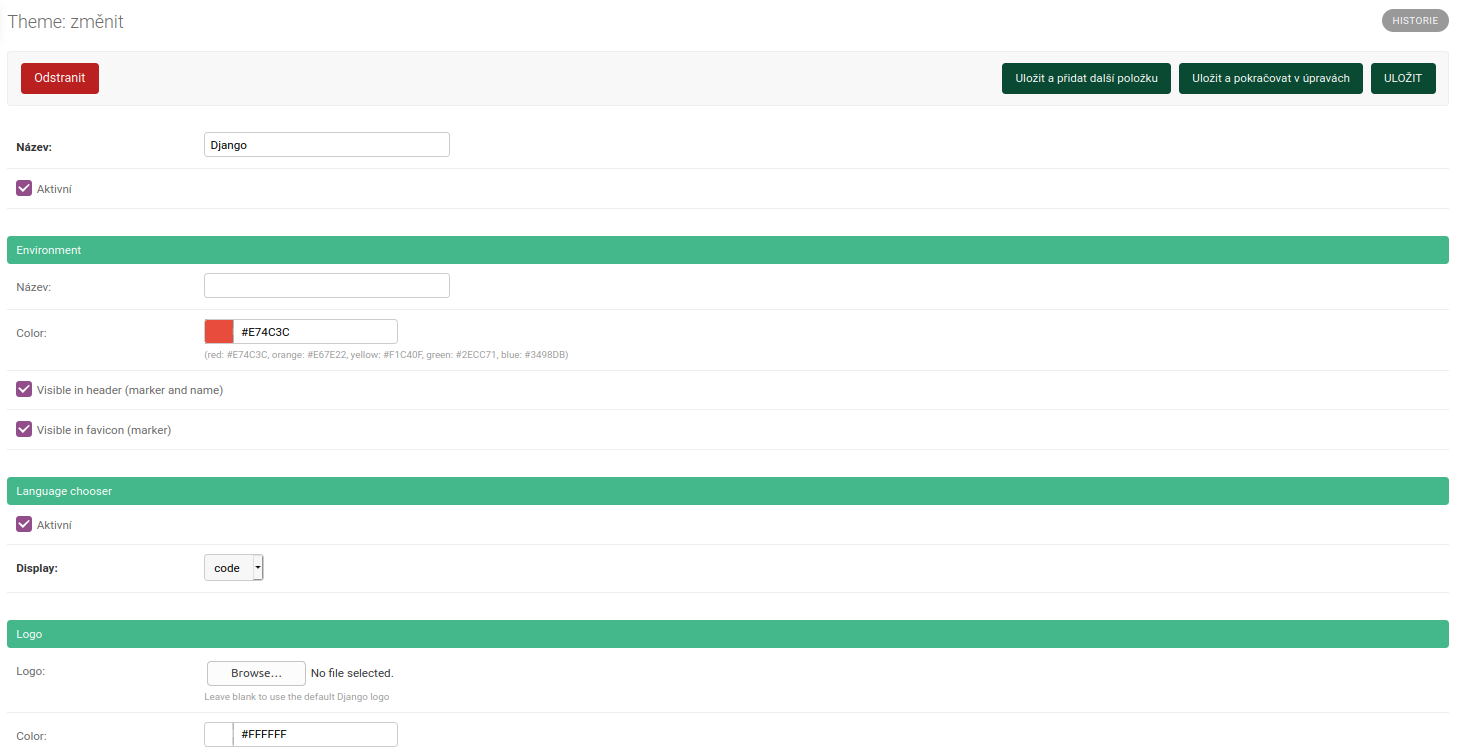
\includegraphics[width=420pt]{./pictures/57-theme.png}
    \caption[Nastavení vzhledu stránky]{Nastavení vzhledu stránky}
	\label{Nastavení vzhledu stránky}                                
\end{figure}



\chapter{Zdrojový kód}
\label{Zdrojový kód}

\begin{itemize}
	\item naki-viskalia.zip
\end{itemize}




% Konec dokumentu
\end{document}
